\chapter{Logarithm}
\textbf{Definition:} A number $x$ is called the logarithm of a number $y$ to the base $b$ if $b^x = y$, where $b > 0, b\neq 1, y > 0$.

\noindent Mathematically, it is represented by the equation $\log_b y = x$ or $b^x = y$.

\textbf{Notes:}
\begin{enumerate}
\item The conditions $b>0, b\neq 1$ and $y>0$ are necessary in the definition of logarithm.
\item When $b=1$ suppose logarithm is defined, and we have to find the value of $\log_1y$. Let
  $\log_1y=x\Rightarrow 1^x=y\Rightarrow 1=y$.

  If $\log_12$ is defined then $1 = 2$. So we see that $b = 1$ leads to meaningless results. Similarly, it is true for $b \neq 1$.
\item Similarly if $y < 0$, then $b^x = y$, which is meaningless as L.H.S. is positive while R.H.S. is negative.
\item Let the condition to be true when $b = 0$. Thus, $0^x = y\Rightarrow 0 = y$. Thus, if $\log_0 2$ is defined then $0 =
  2$. Hence, our assumption leads to failure.
\item No number can have two different logarithms to a given base. Assume that a number $N$ has two different logarithms $x$ and
  $y$ with base $b$. Then, $\log_b N = x$ and $\log_b N = y$

  $\Rightarrow N = b^x$ and $N = b^y$

  $\Rightarrow b^x = b^y \Rightarrow x = y$
\item When the number or base is negative the value of logarithm comes out to be a complex number with non-zero imaginary part.

  Let $\log_e(-5) = x \Rightarrow \log_e(5.e^{i\pi}) = x$ (In complex numbers $e^{i\pi} = -1$)

  $x = \log_e5 + i\pi$
\end{enumerate}

\section{Important Results}
\begin{enumerate}
\item $\log_b 1 = 0$

  \textbf{Proof:} Let $\log_b 1 = x\Rightarrow b^x = 1 \Rightarrow x = 0$
\item $\log_b b = 1$

  \textbf{Proof:} Let $\log_b b = x \Rightarrow b^x = b \Rightarrow x = 1$
\item $b^{\log_b N} = N$

  \textbf{Proof:} Let $\log_b N = x\Rightarrow b^x = N \Rightarrow b^{\log_b N} = N$
\end{enumerate}
\section{Important Formulas}
\begin{enumerate}
\item $\log_b(x.y) = \log_bx + \log_by, (x>0, y>0)$

  \textbf{Proof:} Let $\log_bx = m \Rightarrow b^m = x$. Similarly, $b^n = y$

  $xy = b^{m + n} = b^o$ (say)

  $m + n = o \Rightarrow \log_b(x.y) = \log_bx + \log_by$

  \textbf{Corollary:} $\log_b(xyz) = \log_bx + \log_by + \log_bz$

  If $x, y < 0,$ then $\log_b(x.y) = \log_b|x| + \log_b|y|$
\item $\log_b\left(\frac{x}{y}\right) = \log_b x - \log_b y, (x, y > 0)$

  \textbf{Proof:} Let $\log_bx = m \Rightarrow b^m = x$ and $\log_by = n \Rightarrow b^n = y$

  $\frac{x}{y} = b^{m - n}$ and $\log_b\left(\frac{x}{y}\right) = o \Rightarrow b^o = \frac{x}{y}$

  $\Rightarrow m - n = o \Rightarrow \log_b\left(\frac{x}{y}\right) = \log_b x - \log_b y$

  $\log_b\left(\frac{x}{y}\right) = \log_b|x| - \log_b|y|, (x, y < 0)$
\item $\log_bN^k = k\log_b N$

  \textbf{Proof:} Let $\log_bN = x \Rightarrow b^x = N$

  Let $\log_bN^k = y \Rightarrow b^y = N^k \Rightarrow b^y = b^{kx} \Rightarrow y = kx$

  $\Rightarrow \log_bN^k = k\log_b N$
\item $\log_ba = \log_ca\log_bc$

  \textbf{Proof:} Let $\log_ba = x \Rightarrow b^x = a$

  $\log_ca = y \Rightarrow c^y = a$

  $\log_bc = z \Rightarrow b^z = c$

  $b^x = a = c^y = b^{yz} \Rightarrow x = yz \Rightarrow \log_ba = \log_ca\log_bc$

  Alternatively, we can also write it as $\log_ba = \frac{\log_ca}{\log_cb}$
\item $\log_{b^k}N = \frac{1}{k}\log_bN[b > 0]$

  \textbf{Proof:} From previous item we can infer that $\log_{b^k}N = \frac{\log N}{\log b^k} = \frac{1}{k}\log_bN$

  $\log_{b^k}N = \frac{1}{k}\log_{|b|}N[b< 0, k = 2m, m\in N]$
\item $\log_ba = \frac{1}{\log_ab}$

  \textbf{Proof:} Let $\log_ba = x \Rightarrow b^x = a$

  Also let $\log_ab = y \Rightarrow a^y = b = a^{xy} \Rightarrow xy = 1$

  $\Rightarrow \log_ba = \frac{1}{\log_ab}$
\end{enumerate}

\section{Bases of Logarthims}
There are two popular bases for logarithms. Common base is $10$ and another is $e$. When base is $10$, logarithm is known as
\textit{common logarithm} and when base is $e$, logarithm is known as \textit{natural} or \textit{Napierian logarithm}.

$\log_{10}x$ is also written as $lg~x$ and $\log_ex$ as $ln~x$.

\section{Characteristics and Mantissa}
Typically a logarithm will have an integral part and a fractional part. The integral part is called \textit{characteristics} and
fractional part is called \textit{mantissa}.

For example, if $\log x = 4.7$ then $4$ is characteristics and $.7$ is mantissa of logarithm. If characteristics is less that zero
then at times it is written with a bar above it. For example, $\log x=-5.3=\overline{5}.3$

As you can easily figure out the number of possitive integers having base $b$ and characteristics $n$ is $b^{n + 1} - b^n$.

\section{Inequality of Logarithms}
If $b > 1$ and $\log_bx_1 > \log_bx_2$ then $x_1 > x_2$. If $b < 1$ and $\log_bx_1 > \log_bx_2$ then $x_1 < x_2$.

\section{Expansion of Logarithm and Its Graph}
The logarithm series is given below:

$$\log(1 + x) = x - \frac{x^2}{2} + \frac{x^3}{3} - \frac{x^4}{4} + \ldots$$

\begin{figure}[H]
\begin{center}
  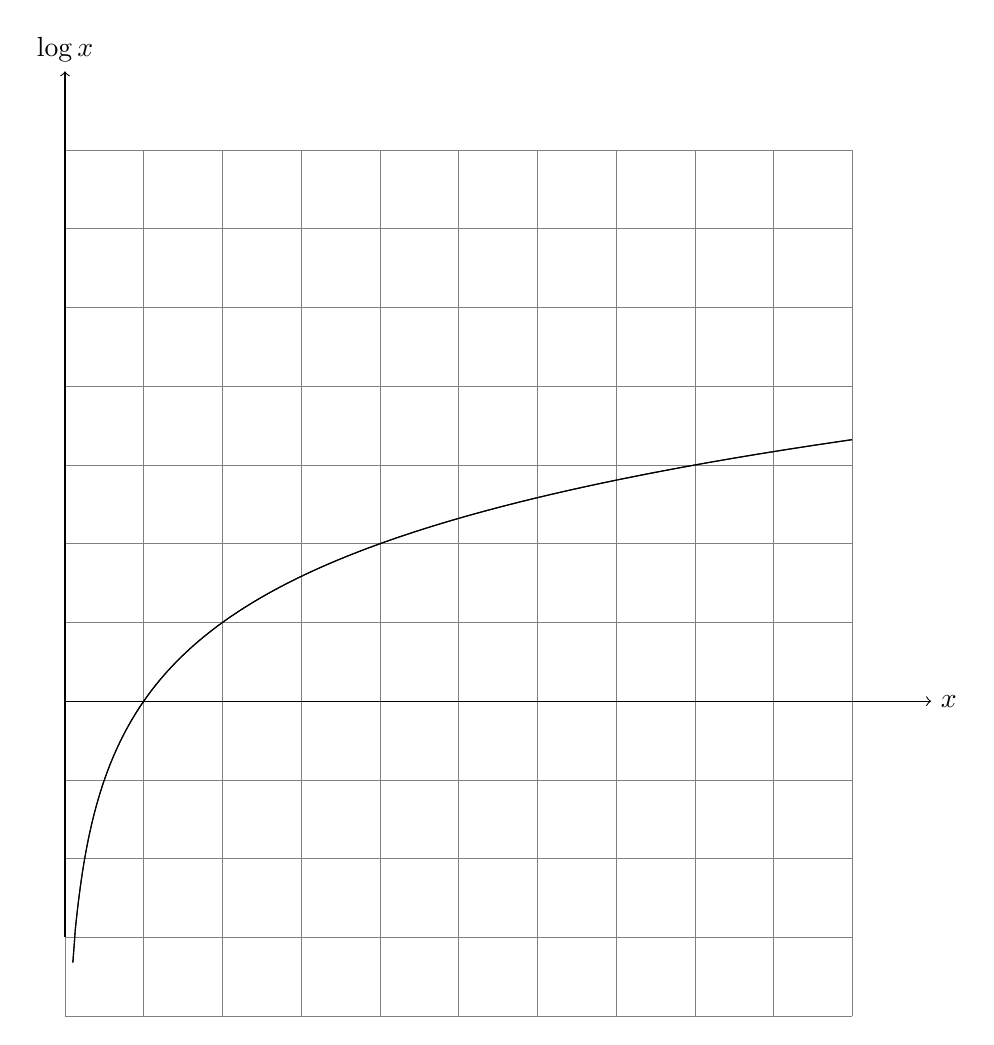
\begin{tikzpicture}
    \draw [help lines] (0,-4) grid [step=1] (10,7);
    \draw (0,0) -- (10,0);
    \draw[->] (0, 0) -- (11, 0) node[right] {$x$};
    \draw[->] (0, -3) -- (0, 8) node[above] {$\log x$};
    \draw plot [domain=0.1:10,samples=1000] (\x,{log2(\x)});
    \draw plot [domain=0.1:10,samples=1000] (\x,{log2(\x)});
  \end{tikzpicture}
  \caption{Graph of $\log 2$}
\end{center}
\end{figure}

So we can see that rate of increment of logarithm function decreases. Rate of increment of logarithm function is given by
$\frac{1}{x}$ at any point $x$, as we will learn when we study Calculus and derivatives.

\section{Problems}
\begin{enumerate}
\item Find the value of $x$, where $\log_{\sqrt{8}} x = \frac{10}{3}$.
\item Prove that $\log_ba.\log_cb.\log_ac = 1$.
\item Prove that $\log_3\log_2\log_{\sqrt{5}}625 = 1$.
\item If $a^2 + b^2 = 23ab$, then prove that $\log\frac{a + b}{5} = \frac{1}{2}(\log a + \log b)$.
\item Prove that $7\log\frac{16}{15} + 5\log\frac{25}{24} + 3\log\frac{81}{80} = \log 2$.
\item Find the value of $\log\tan1^\circ + \log\tan2^\circ + \ldots + \log\tan89^\circ$.
\item Evaluate $\log_9\tan\frac{\pi}{6}$.
\item Evaluate $\frac{\log_{a^2}b}{\log_{\sqrt{a}}b^2}$.
\item Evaluate $\log_{\sqrt{5}}.008$.
\item Evaluate $\log_{2\sqrt{3}}144$.
\item Prove that $\log_3\log_2\log_{\sqrt{3}}81 = 1$.
\item Prove that $\log_ax\log_by = \log_bx\log_ay$.
\item Prove that $\log_2\log_2\log_216 = 1$.
\item Prove that $\log_ax = \log_bx\log_cb\ldots\log_nm\log_an$.
\item Prove that $a^x = 10^x\log_{10}a$.
\end{enumerate}
